%!TEX root = main.tex
\chapter{Applications of Parameter Estimation and Inference}\label{ch:parameter2}

\section{Normal Model - Inference about Means}

\example{Iris petal lengths - Best estimate}

\begin{table}
\begin{center}
\begin{tabular}{ccccc}
\toprule
1.4& 1.4& 1.3& 1.5& 1.4\\
1.7& 1.4& 1.5& 1.4& 1.5\\
1.5& 1.6& 1.4& 1.1& 1.2\\
1.5& 1.3& 1.4& 1.7& 1.5\\
1.7& 1.5& 1.0& 1.7& 1.9\\
1.6& 1.6& 1.5& 1.4& 1.6\\
1.6& 1.5& 1.5& 1.4& 1.5\\
1.2& 1.3& 1.5& 1.3& 1.5\\
1.3& 1.3& 1.3& 1.6& 1.9\\
1.4& 1.6& 1.4& 1.5& 1.4\\
\bottomrule
\end{tabular}
\end{center}
\label{tbl:iris_length}
\caption{Iris petal lengths, in centimeters, for Iris type \emph{Setosa}.}
\end{table}

Table~\ref{tbl:iris_length} shows data for the lengths (in centimeters) of the petals of one species of Iris flower\cite{Bache:2013fk}.  If we want to estimate the ``true'' length of the the petal for this species, given all of these examples, we would apply the following model of the data:
\begin{marginfigure}
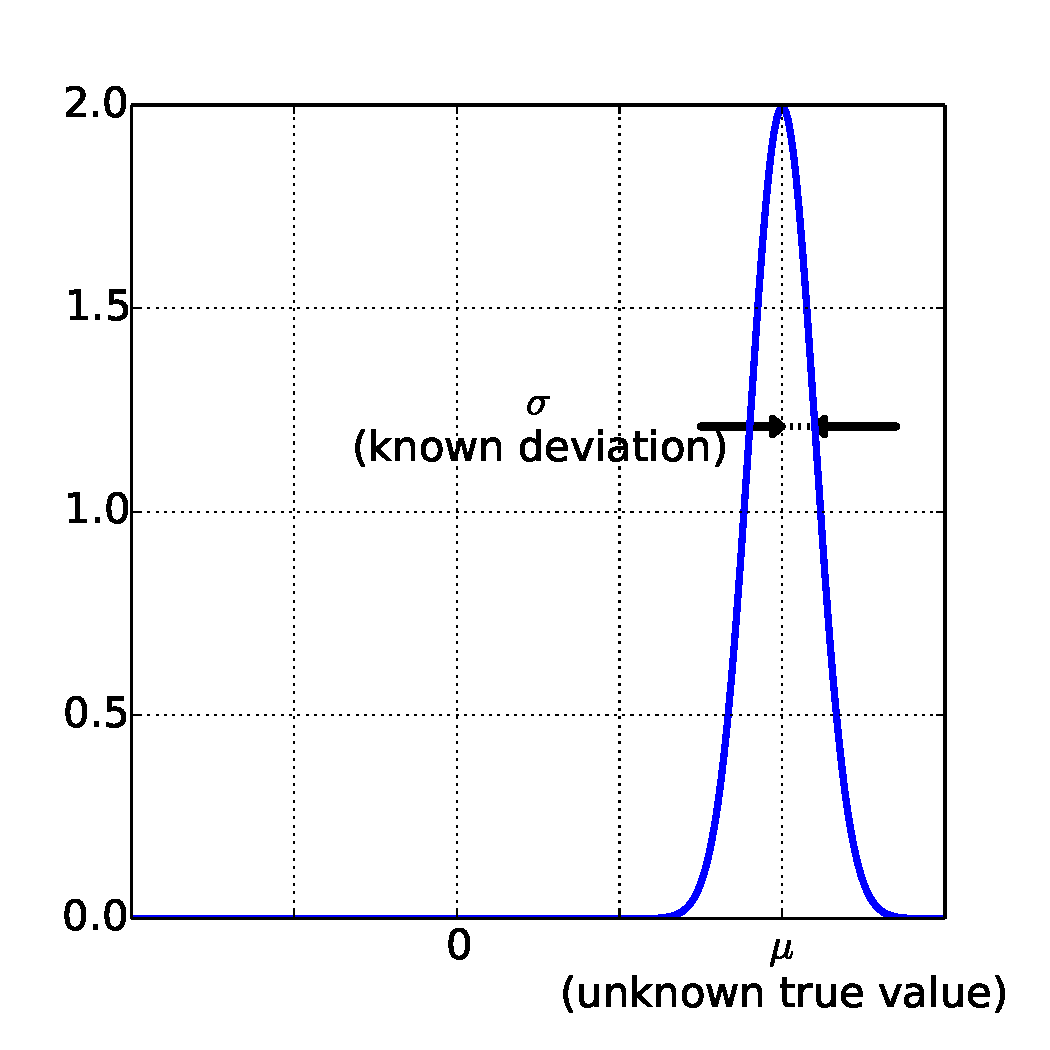
\includegraphics{normal_mu_known_sigma}
\end{marginfigure}

\beqn
{\rm data} &=& \mbox{true value} + \mbox{Normal(mean=0,known $\sigma$)}
\eeqn
or equivalently
\beqn
{\rm data} &=& \mbox{Normal(mean=\mbox{true value},known $\sigma$)}
\eeqn
The resulting distribution for the ``true value'', $\mu$, is also a {\em Normal} distribution (Section~\ref{sec:estmean}),
\beqn
P(\mu|{\rm data},\sigma) = {\rm Normal}(\bar{x}, \sigma/\sqrt{N})
\eeqn 
where the best estimate of the true value, $\mu$ is the sample mean, $\bar{x}$, and the uncertainty is related to the sample deviation (which we're going to take as the ``known'' deviation, $\sigma \sim  0.174$) in this case. Thus,
\beqn
\hat{\mu}&=&\bar{x}=\frac{1.4+1.4+1.3+1.5+\cdots+1.6+1.4+1.5+1.4}{50}\\
&=&1.464
\eeqn
and the full answer, with uncertainty, is 
\beqn
\hat{\mu}&=&1.464 [{\rm cm}] \pm \frac{0.174}{\sqrt{50}}[{\rm cm}] \\
&=& 1.464 [{\rm cm}] \pm 0.025 [{\rm cm}]
\eeqn

\example{Iris petal lengths - A different species?}

Here we apply the $z$-test (Section~\emph{\nameref{sec:ztest}} on page~\pageref{sec:ztest}) to a new observation to see if there is reason to believe it to be a different species.  Imagine we have a single observation of another iris with petal length 2.5 [cm].  Is this likely to be the same type as the {\em Setosa} type above?    As outlined in Section~\ref{sec:sumdiffnormal}, we get the best estimate for the difference as:
\beqn
\mu_{\rm diff} = 2.5 - 1.464 = 1.036
\eeqn
with uncertainty the same as the uncertainty of the {\em Setosa} type, so the final estimate with uncertainty is:
\beqn
1.036 [{\rm cm}] \pm 0.025 [{\rm cm}]
\eeqn
which is 
\beqn
\frac{1.036 [{\rm cm}]}{0.025 [{\rm cm}]} = 41 \mbox{ deviations away from zero!}
\eeqn
which makes it \emph{virtually certain} to be a different type (see Table~\ref{tbl:norm likely}).


\section{Normal Model Again - Inference about Means and Deviations}

\begin{table}
\begin{center}
\begin{tabular}{cccccc}
\toprule
{\it Setosa} &1.4& 1.4& 1.3& 1.5& 1.4\\
{\it Virginica} & 6.0& 5.1& 5.9& 5.6& 5.8\\
{\it Versicolor} &4.7& 4.5& 4.9& 4.0& 4.6\\
\bottomrule
\end{tabular}
\end{center}
\label{tbl:iris_length2}
\caption{Subset of iris petal lengths, in centimeters, for iris types~\emph{Virginica}, \emph{Setosa}, and \emph{Versicolor}.}
\end{table}

\example{Iris petal lengths - Significantly different?}

In this example we apply the $t$-test (Section~\emph{\nameref{sec:ttest}} on page~\pageref{sec:ttest}) to a subset of the iris samples, to see if the different species can be reasonably separated using their petal lengths.  Shown in Table~\ref{tbl:iris_length2} is a very small subset of the full iris petal-length data.  Are the types \emph{Virginica} and \emph{Versicolor} longer than the type \emph{Setosa}?  Is the \emph{Virginica} longer than \emph{Versicolor}?  For each of these, we need to specify the model, determine the best estimate for the parameters of the model, and then compare the distributions.

The model we will use is the simple Normal model, 
\beqn
{\rm data} &=& \mbox{Normal(mean=\mbox{true value},unknown $\sigma$)}
\eeqn
which is the same as the previous example, except that the deviation, $\sigma$, is unknown.  In addition to being unknown, there are so few data points that the deviation can't be well approximated with the sample deviation.  

The resulting distribution for the ``true value'', $\mu$, is a {\em Student-t} distribution (Section~\ref{sec:meansigmaest}),
\beqn
P(\mu|{\rm data}) = {\rm Student}_{{\rm dof}=N-1}(\bar{x}, S/\sqrt{N})
\eeqn 
The best estimates for the true length-values of each type is given by their sample means, 
\beqn
\hat{\mu}_{\rm setosa}=\frac{1.4+1.4+1.3+1.5+1.4}{5}=1.40 \\
\hat{\mu}_{\rm virginica}=\frac{6.0+5.1+5.9+5.6+5.8}{5}=5.68 \\
\hat{\mu}_{\rm versicolor}=\frac{4.7+4.5+4.9+4.0+4.6}{5}=4.54
\eeqn
and the sample deviations for each is given by


\beqn
S_{\rm setosa}&=&\sqrt{\frac{1}{5-1}\cdot\left((1.4-1.40)^{2}+(1.4-1.40)^{2}+(1.3-1.40)^{2}+(1.5-1.40)^{2}+(1.4-1.40)^{2}\right)} \\
&=&=0.07\\
S_{\rm virginica}&=&\sqrt{\frac{1}{5-1}\cdot\left((6.0-5.68)^{2}+(5.1-5.68)^{2}+(5.9-5.68)^{2}+(5.6-5.68)^{2}+(5.8-5.68)^{2}\right)}\\
&=&=0.36\\
S_{\rm versicolor}&=&\sqrt{\frac{1}{5-1}\cdot\left((4.7-4.54)^{2}+(4.5-4.54)^{2}+(4.9-4.54)^{2}+(4.0-4.54)^{2}+(4.6-4.54)^{2}\right)}\\
&=&0.34
\eeqn

The posterior probability distributions, shown in Figure~\ref{fig:iris_tdist}, have the following form:
\beqn
P(\mu_{\rm setosa}|{\rm data}) &=& {\rm Student}_{{\rm dof}=4}(1.40, 0.07/\sqrt{5})\\
P(\mu_{\rm virginica}|{\rm data}) &=& {\rm Student}_{{\rm dof}=4}(5.68, 0.36/\sqrt{5})\\
P(\mu_{\rm versicolor}|{\rm data}) &=& {\rm Student}_{{\rm dof}=4}(4.64, 0.34/\sqrt{5})
\eeqn 
It is clear from the picture that they are very well separated, but we can quantify this by looking at the probability that the difference between their means is greater than zero.

\begin{figure}
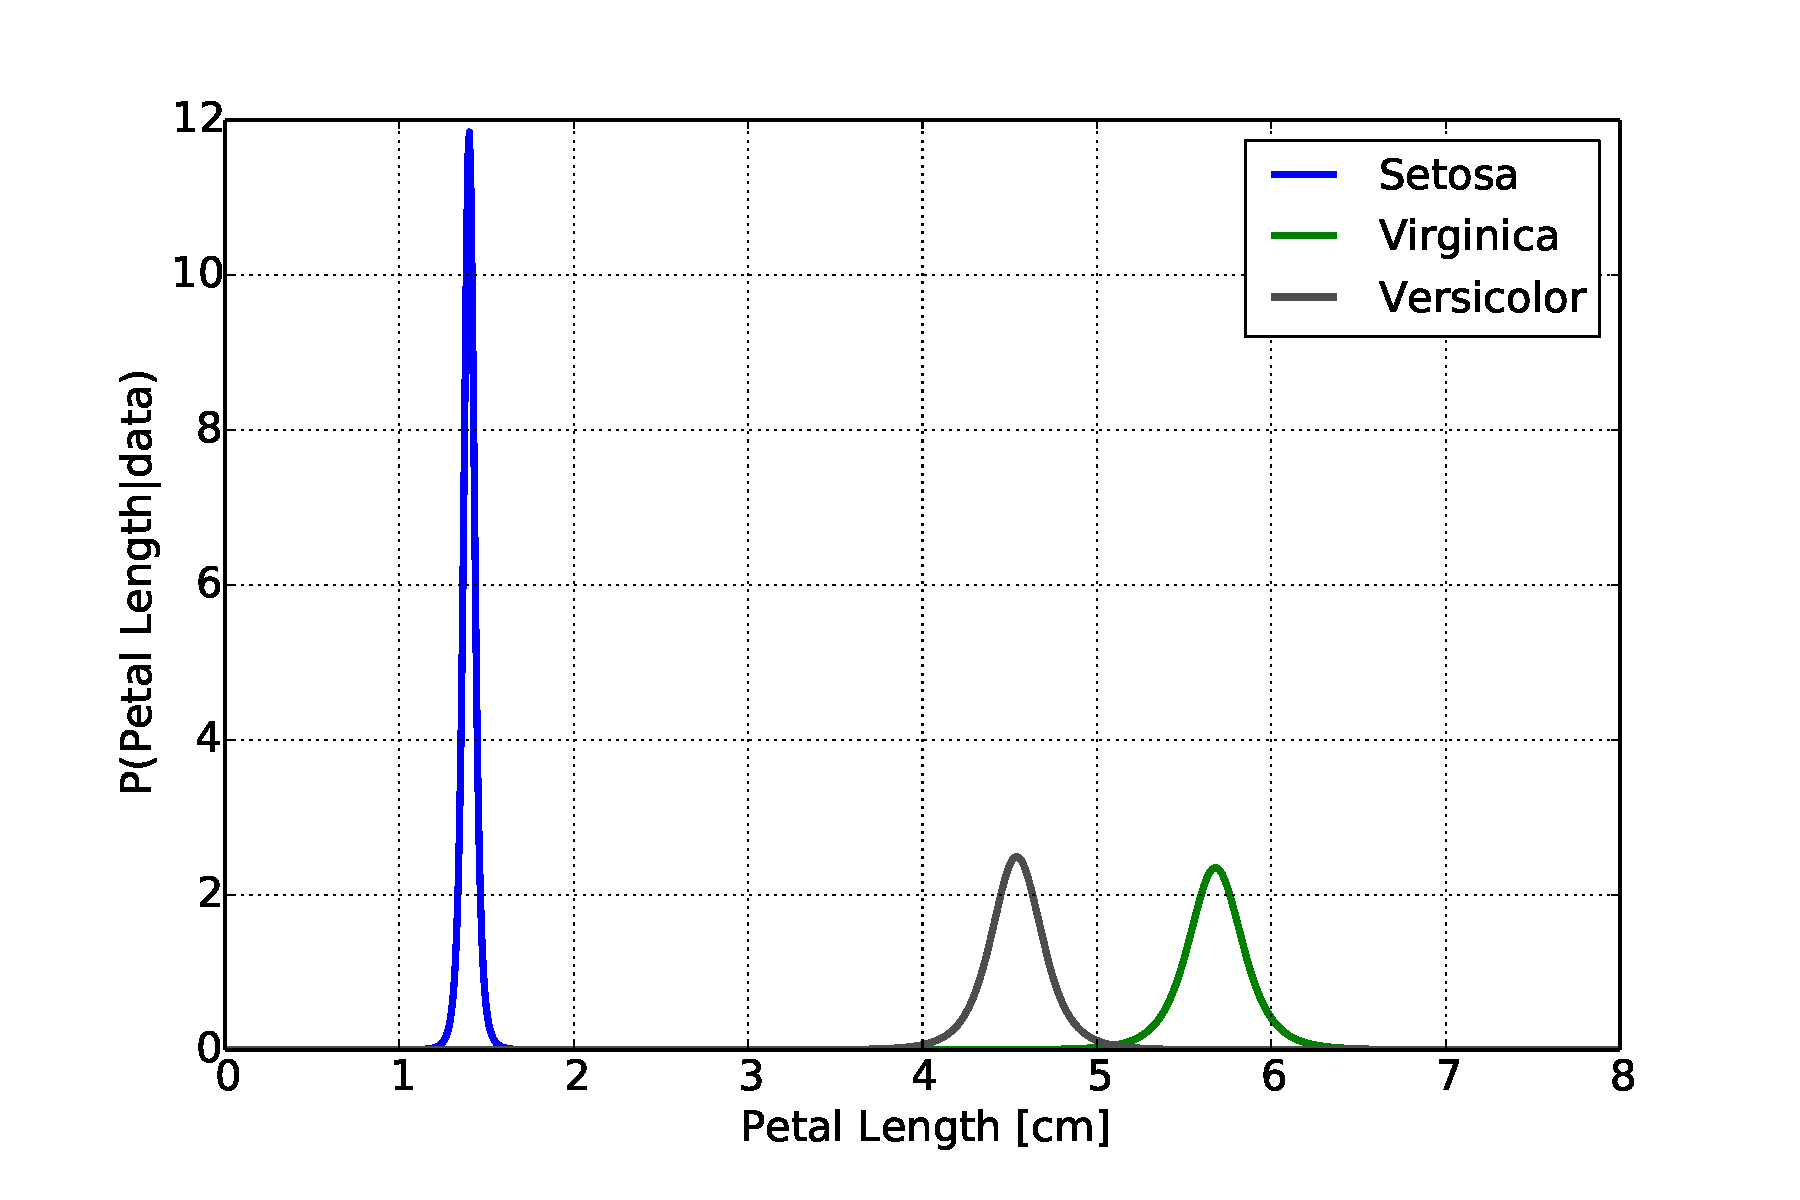
\includegraphics{iris_tdist}
\caption{Probability distributions for the subset of iris petal lengths.  Each distribution follows a Student-t form.}
\label{fig:iris_tdist}
\end{figure}

The probability of their difference approximately\marginnote{This approximation is called Welch's method.  The exact analysis is beyond this book, but numerically one can calculate it and it doesn't differ from this approximate analysis in any significant way.  Essentially you calculate $P(\mu_{\rm versicolor}>\mu_{\rm virginica}|{\rm data})$ by adding up the $P(\mu_{\rm versicolor}|{\rm data})\times P(\mu_{\rm virginica}|{\rm data})$ for all possible lengths where  versicolor is longer than virginica.} takes the form of a Student's {\em t} distribution, with the same center and deviation shown for the Normal in Section~\ref{sec:sumdiffnormal}.  Here we do the calculation between the closest two iris types, \emph{Virginica} and \emph{Versicolor}:
\beqn
\mu_{\rm diff}&=&5.68-4.64 = 1.04 \\
\sigma_{\rm diff}&=& \sqrt{\frac{0.36^{2}}{5}+\frac{0.34^{2}}{5}} = 0.22
\eeqn
The degrees of freedom used for this Student's {\em t} distribution is approximately the smallest one from the two samples, or in this case (since both samples have the same number of data points), dof=4.  The resulting posterior probability distribution for the difference of means is shown in Figure~\ref{fig:iris_tdist_diff}.  

We observe that the difference of the means is over 4 times the deviation away from zero, so even with 4 degrees of freedom, this is significant at the 99\% level. We can be highly certain that these two species have different petal lengths, and that the difference observed is not just a product of the random sample. 

\begin{figure}
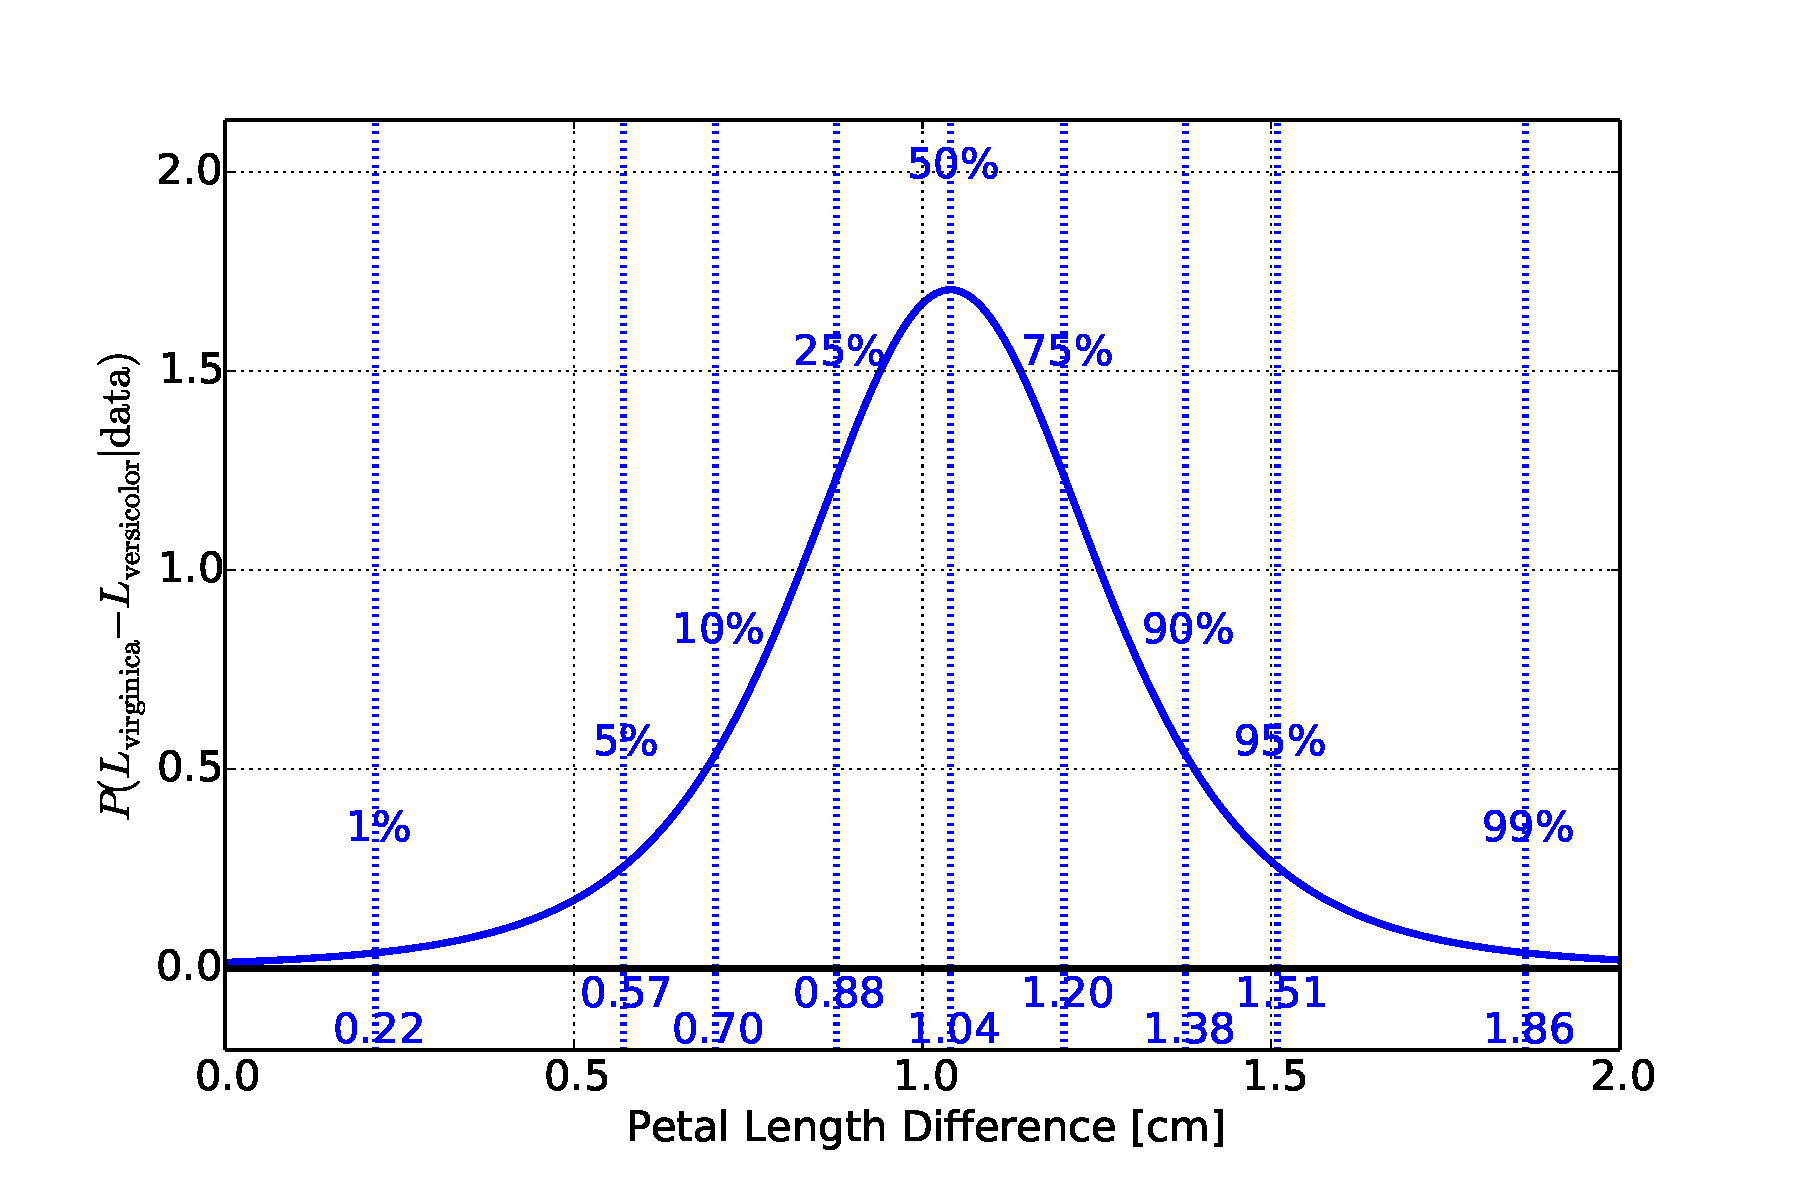
\includegraphics{iris_tdist_diff}
\caption{Probability distributions for the difference between iris petal lengths for the closest two iris types, \emph{Virginica} and \emph{Versicolor}.  The distribution follows a Student-t form, and clearly shows significant probability (greater than 99\%) for being greater than zero.}
\label{fig:iris_tdist_diff}
\end{figure}



\example{Ball Bearing Sizes}

Here's a data data set, measuring the size of ball bearings\cite{hand2011handbook}  from two different production lines.

\begin{table}
\begin{center}
\begin{tabular}{cccccccccc}
\toprule
\multicolumn{9}{c}{\em First line [microns]}\\
1.18& 1.42& 0.69& 0.88& 1.62& 1.09& 1.53& 1.02& 1.19& 1.32 \\
\multicolumn{9}{c}{\em Second line [microns]} \\
1.72& 1.62& 1.69& 0.79& 1.79& 0.77& 1.44& 1.29& 1.96& 0.99\\
\bottomrule
\end{tabular}
\end{center}
\label{tbl:ball_bearing}
\caption{ Production lines are produce a ball bearing with a diameter of approximately 1 micron. Ten ball bearings were randomly picked from the production line (i.e. the \emph{First line}) at one time, and then again for a different production line (i.e. the \emph{Second line}). Romano, A. (1977) \emph{Applied Statistics for Science and Industry}.}
\end{table}

We can ask questions such as:
\bi
\i What is our best estimate of the size of a ball bearing, given one of the production lines?
\i Is it reasonable to believe that there is a difference in the size produced between the two lines?
\ei

\example{What is the best estimate (and uncertainty) for each of the two production lines of ball bearings?}

Using the normal approximation to the Student-T distribution (Section~\ref{sec:normal_t_approx}), we have the best estimates of the two lines as
\beqn
\mu_{1}&=&\frac{1.180000 + 1.420000 + 0.690000 + \cdots + 1.190000 + 1.320000}{10} \\
&=&1.194
\eeqn
\beqn
\mu_{2}&=& \frac{1.720000 + 1.620000 + 1.690000 + \cdots + 1.960000 + 0.990000}{10}\\
&=&1.406
\eeqn
and their uncertainties calculated by first calculating the sample deviations
\beqn
S_{1}&=&\sqrt{\frac{1}{10-1}\cdot \left((1.18-1.194)^2 + (1.42-1.194)^2 + \cdots + (1.19-1.194)^2 + (1.32-1.194)^2\right)} \\
&=&0.289\\
S_{2}&=&\sqrt{\frac{1}{10-1}\cdot \left((1.72-1.406)^2 + (1.62-1.406)^2 + \cdots + (1.96-1.406)^2 + (0.99-1.406)^2\right)} \\
&=&0.428
\eeqn
and then scaling the deviations by the number of data points
\beqn
\sigma_{1}&=&S_{1}/sqrt{10} = 0.092 \\
\sigma_{2}&=&S_{2}/sqrt{10} = 0.135
\eeqn
yielding the best estimates and uncertainties for the two production lines
\bi
\i Production line 1: 1.194 [microns]$\pm$ 0.092[microns]
\i Production line 2: 1.406 [microns]$\pm$ 0.135[microns]
\ei
or looking at the 95\% CI for each line\marginnote{This is just the $\pm 2\cdot \sigma$ range}
\bi
\i Production line 1: 1.01[microns] - 1.378[microns]
\i Production line 2: 1.136[microns] - 1.676[microns]
\ei
Roughly, given that these intervals overlap, there is not strong evidence that there is a difference between the two lines.

\example{Is it reasonable to believe that there is a difference in the size produced between the two lines?}

Using the best estimate of the difference, we get
\beqn
\delta_{12} = \mu_{2}-\mu_{1} = 0.212
\eeqn
with the uncertainty in the difference from the individual uncertainties,
\beqn
\sigma_{12} &=& \sqrt{\sigma_{1}^{2}+\sigma_{2}^{2}} = 0.163
\eeqn

So the $2\cdot \sigma$ uncertainty range for the difference, 
\beqn
[0.212-2\cdot 0.163,0.212+2\cdot 0.163] = [-0.114,0.538]
\eeqn
includes the value zero, which we interpret as a statement that the difference is \emph{not statistically significant}.  In other words, it is \emph{not reasonable} to believe that there is a difference in the size produced between the two lines.

\section{Beta Model - Inference About Proportions}

\example{The Sunrise Problem}

The sunrise problem, as first stated by Laplace, is ``What is the probability that the sun will rise tomorrow?''  We'll start with the assumption that initially one has never seen a sunrise, and then observe a year of sunrises each morning with no morning without one.  Thus we have the form of the data as $h$ successes (days with a sunrise) in $N$ total days.  Our model of the data is specified as before with a binomial distribution, resulting in the posterior Beta, as described in Section~\ref{sec:bestest}.  

After a only 10 years of watching sunrises, and no failures of a sunrise, the best estimate for the probability of a sunrise is
\beqn
\hat{\theta}_{\rm median}&\approx&\frac{h+2}{N+4} \\
&=&\frac{3650+2}{3650+4}=0.9995\\
\eeqn
making it virtually certain for a sunrise.  


\example{Cancer Rates}

This example is from Donald Berry's Statistics textbook\cite{berry1996statistics}:
\begin{quote}
pp 192: A study (Murphy and Abbey, Cancer in Families, 1959) addressed the question of whether cancer runs in families. The investigator identified 200 women with breast cancer and another 200 women without breast cancer and asked them whether their mothers had had breast cancer. Of the 400 women in the two groups combined, 10 of the mothers had had breast cancer. If there is no genetic connection, then about half of these 10 would come from each group.
\end{quote} 
The data is that 7 of the daughters had cancer and 3 did not. Is there strong evidence of a connection?

The proper way, assuming total initial ignorance, is to use the Beta distribution:
\beqn
\Pg{$\theta_{\rm cancer}$}{data}= {\rm Beta}(h=7,N=10)
\eeqn
which has a median of $\hat{\theta}_{\rm cancer}=0.68$, but a 95\% credible interval of $\hat{\theta}_{\rm cancer}=0.39$ up to $\hat{\theta}_{\rm cancer}=0.89$.  This means there is not strong evidence of an effect.

\example{Cancer Rates - Normal Approximation}

We can estimate the the Beta distribution median and credible intervals with a Normal distribution, by using the ``assuming 2 successes and 2 failures'' method.
\beqn
\hat{\theta}_{\rm cancer}&=&\frac{h+2}{N+4} \\
&=&\frac{7+2}{10+4}= 0.643
\eeqn
and
\beqn
\sigma&=&\sqrt{\hat{\theta}_{\rm cancer}(1-\hat{\theta}_{\rm cancer})/(N+4)} \\
&=&\sqrt{0.643 (1-0.643)/(10+4)}\\
&=&0.128
\eeqn
So the approximate 95\% credible interval is
\beqn
\hat{\theta}_{\rm cancer}\pm 2\sigma
\eeqn
which is between 0.387 and 0.899, again with the same conclusion of no strong evidence of an effect.


\example{Will it rain on the 4$^{\rm th}$ of July?}

In the United States, the 4$^{\rm th}$ of July is Independence Day, and is known for parades.  The oldest continuously running parade is in Bristol, RI, and it runs rain or shine.  Is it likely to rain on the parade?  Climate data from nearby Providence is here from wunderground.com:

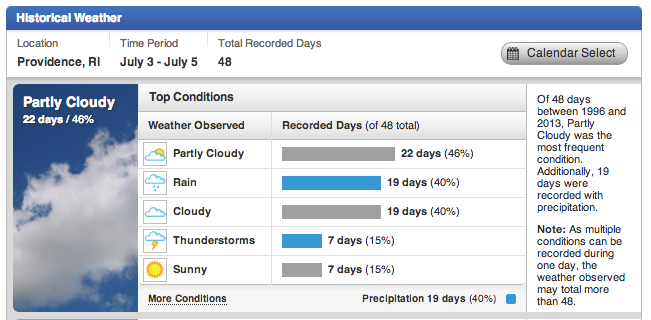
\includegraphics{average_weather_jul4_prov.png}

We can estimate the the Beta distribution median and credible intervals with a Normal distribution, by using the ``assuming 2 successes and 2 failures'' method.
\beqn
\hat{\theta}_{\rm rain}&=&\frac{h+2}{N+4} \\
&=&\frac{19+2}{48+4}= 0.404
\eeqn
around 40\%, less than an even chance (50\%) of rain, but
\beqn
\sigma&=&\sqrt{\hat{\theta}_{\rm rain}(1-\hat{\theta}_{\rm rain})/(N+4)} \\
&=&\sqrt{0.404 (1-0.404)/(48+4)}\\
&=&0.068
\eeqn
So the approximate 95\% credible interval is
\beqn
\hat{\theta}_{\rm rain}\pm 2\sigma
\eeqn
which is between 0.268 and 0.540.  This is not strong evidence against a purely fair and random ``coin flip'' for rain on the 4$^{\rm th}$ of July.


\example{Hot Hand Reexamined\label{ex:hothand}}

In Tversky and Gilovich\cite{tversky2005cold} we have the following data for Larry Bird free throws in basketball:
\bi
\i Given each of 53 missed shots, Larry Bird successfully shot 48 of the \emph{next} attempt.
\i Given each of 285 successful shots, Larry Bird successfully shot 251 of the \emph{next} attempt.
\ei

This data alone almost suggests an anti-hot-hand (where you're \emph{less} likely to make a successful attempt following a successful shot).  However, we can demonstrate that these numbers are not in fact statistically different.  Given the relatively large number of attempts (greater than 30) we can use the Normal approximation to estimate the two probabilities of success:
\beqn
\theta_{\mbox{after a miss}} &=& \frac{48+2}{53+4} = 0.877\\
\theta_{\mbox{after a success}} &=& \frac{251+2}{285+4} = 0.875
\eeqn
and the uncertainty,
\beqn
\sigma_{\mbox{after a miss}} &=& \sqrt{0.877 (1-0.877)/(53+4)}=0.044\\
\sigma_{\mbox{after a success}} &=& \sqrt{0.875 (1-0.875)/(285+4)=0.019}
\eeqn
making the 95\% credible intervals for probability of a Larry Bird successful attempt
\beqn
95\% {\rm CI}_{\mbox{after a miss}}&=&0.877\pm 2\cdot 0.044 = [0.789,0.965]\\
95\% {\rm CI}_{\mbox{after a success}}&=&0.875\pm 2\cdot 0.019 = [0.837,0.913]
\eeqn
Notice that the intervals overlap, so there is no significant evidence for a difference in Larry Bird's success following another success or following a miss.  Thus, there is no significant evidence for a hot hand, or an anti-hot hand.

\section{Model Construction}

In practice, we either don't know what the optimum model we need is, or the needs of the model change as we obtain more data.  

We start with the data in Table~\ref{tbl:penny1} for the mass of pennies of various years (shown graphically in Figure~\ref{fig:penny1})\footnote{this data was extracted from student measurements during a physics lab}:
\begin{table}
\begin{center}
\begin{tabular}{ccccc}
\toprule
{\bf Year} & {\bf Mass [g]} \\
1960& 3.133\\
1961& 3.083\\
1962& 3.175\\
1963& 3.120\\
1964& 3.100\\
1965& 3.060\\
1966& 3.100\\
1967& 3.100\\
1968& 3.073\\
1969& 3.076\\
1970& 3.100\\
1971& 3.110\\
1972& 3.080\\
1973& 3.100\\
1974& 3.093\\
\bottomrule
\end{tabular}
\end{center}
\caption{Mass of Pennies from 1960 to 1974.}
\label{tbl:penny1}
\end{table}

\begin{figure}
\psx{figs/mass1960_1974}{6in}
\caption{Mass of Pennies from 1960 to 1974.}\label{fig:penny1}
\end{figure}

We are going to ignore the measurement uncertainties in these individual measurements, because they are quite small.

\example{Mass of the Penny, Model 1 - One True Value}

If we assume a model that states that there is a ``true'' value and the variation from this ``true'' value caused by some unknown process, but with known magnitude, $\sigma$,
\beqn
{\rm data} &=& \mbox{true value} + \mbox{Normal(mean=0,known $\sigma$)}
\eeqn
or equivalently
\beqn
{\rm data} &=& \mbox{Normal(mean=\mbox{true value},known $\sigma$)}
\eeqn
we can get the best estimate and uncertainty in that estimate from the following procedure, Using the normal approximation to the Student-T distribution (Section~\ref{sec:normal_t_approx}):
\beqn
\hat{\mu}&=&\bar{x} \pm k\cdot S/\sqrt{N}
\eeqn
where the symbols in this equation are
\be
\i the number of data points, $N$.
\i the best estimate for the true value, $\hat{\mu}$, is given by the \emph{sample mean}, $\bar{x}$:
\beqn
\bar{x} &=&= \frac{x_{1}+x_{2}+\cdots+ x_{N}}{N} \\
&=& \frac{3.133 {\rm g} + 3.083 {\rm g}+\cdots + 3.093 {\rm g}}{15} \\
&=& 3.100 {\rm g}
\eeqn
\i The uncertainty is directly related to the \emph{sample standard deviation}, $S$:
\beqn
S&=&\sqrt{\frac{(x_{1}-\bar{x})^{2}+(x_{2}-\bar{x})^{2}+\cdots+(x_{N}-\bar{x})^{2}}{N-1}} \\
&=& \sqrt{\frac{(3.133{\rm g}-3.100 {\rm g})^{2}+(3.083-3.100 {\rm g})^{2}+\cdots+(3.093-3.100 {\rm g})^{2}}{14}} \\
&=& 0.0278 {\rm g}
\eeqn
\i The scale factor, $k$, adjusts for the small number of data points - there is more uncertainty in our estimate when there are fewer data points:
\beqn
k&=& 1+\frac{20}{N^{2}} \\
&=& 1+\frac{20}{15^{2}} \\
&=& 1.0889
\eeqn
\ee

Finally, we have the best estimate and uncertainty for the pennies in this dataset:
\beqn
\hat{\mu}&=&\bar{x} \pm k\cdot S/\sqrt{N} \\
&=& 3.100 {\rm g} \pm 1.0889 \cdot 0.0278 {\rm g}/\sqrt{15} \\
&=& 3.100 {\rm g} \pm 0.0078  {\rm g}
\eeqn
or, as a 99\% credible range (3 times the uncertainty written above), we have, (see also Figure~\ref{fig:penny1_CI})

\beqn
\mbox{99\% CI for } \mu&=& 3.100 {\rm g} \pm 3\times 0.0078  {\rm g} \\
&=&[3.077 {\rm g}, 3.124 {\rm g}]
\eeqn

\begin{figure}
\cc{\psx{figs/mass1965_1974_1_value}{6in}}
\cc{\psx{figs/mass1965_1974_1_value_dist}{6in}}
\caption{Mass of Pennies from 1960 to 1974, with best estimates and 99\% CI (i.e. $3\sigma$) uncertainty.}\label{fig:penny1_CI}
\end{figure}


\example{Mass of the Penny, Model 1 - One True Value with More Data}

Now we collect the additional data with more recent pennies shown in Table~\ref{tbl:penny2}. We can follow the same procedure, assuming our original model of one ``true'' value, to get the best estimate and uncertainty for this model, combining the two data sets.


\begin{table}
\begin{center}
\begin{tabular}{ccccc}
\toprule
{\bf Year} & {\bf Mass [g]} \\
1989& 2.516\\
1990& 2.500\\
1991& 2.500\\
1992& 2.500\\
1993& 2.503\\
1994& 2.500\\
1995& 2.497\\
1996& 2.500\\
1997& 2.494\\
1998& 2.512\\
1999& 2.521\\
2000& 2.499\\
2001& 2.523\\
2002& 2.518\\
2003& 2.520\\
\bottomrule
\end{tabular}
\end{center}
\caption{Mass of Pennies from 1989 to 2003.}
\label{tbl:penny2}
\end{table}


\beqn
\hat{\mu}&=&\bar{x} \pm k\cdot S/\sqrt{N}
\eeqn
where the symbols in this equation are
\be
\i the number of data points, $N=30$.
\i the best estimate for the true value, $\hat{\mu}$, is given by the \emph{sample mean}, $\bar{x}$:
\beqn
\bar{x} &=& \frac{3.133 {\rm g} + 3.083 {\rm g}+\cdots + 2.520 {\rm g}}{30} \\
&=& 2.804 {\rm g}
\eeqn
\i The \emph{sample standard deviation}, $S$:
\beqn
S&=& \sqrt{\frac{(3.133{\rm g}-2.804 {\rm g})^{2}+(3.083-2.804 {\rm g})^{2}+\cdots+(2.520-2.804 {\rm g})^{2}}{29}} \\
&=& 0.3024 {\rm g}
\eeqn
\i The scale factor, $k$, adjusting for the small number of data points:
\beqn
k&=& 1+\frac{20}{30^{2}} \\
&=& 1.0222
\eeqn
\ee

Finally, we have the best estimate and uncertainty for the pennies in this full dataset:
\beqn
\hat{\mu}&=&\bar{x} \pm k\cdot S/\sqrt{N} \\
&=& 2.804 {\rm g} \pm 1.0222 \cdot 0.3024 {\rm g}/\sqrt{30} \\
&=& 2.804 {\rm g} \pm 0.0564  {\rm g}
\eeqn
or, as a 99\% credible range (3 times the uncertainty written above), we have,

\beqn
\mbox{99\% CI for } \mu&=& 2.804 {\rm g} \pm 3\times 0.0564  {\rm g} \\
&=&[2.634 {\rm g}, 2.973 {\rm g}]
\eeqn

There are several things one should notice:
\be
\i The scale factor, $k$, is less for 30 data points than it is for 15 data points.  This is because the adjustment for small number of data points gets less relevant as we obtain more data.  This is what we expect.
\i Despite there being twice as much data, our uncertainty \emph{increased}.  This is unusual, if our model is correct - more data should \emph{sharpen} the estimates.  Although it is possible that adding more data increased the system variability somehow, it is more likely that some assumption of our model is incorrect.  This becomes obvious when we look at the result graphically, shown in Figure~\ref{fig:penny2}.
\ee

\begin{figure}
\cc{\psx{figs/mass1965_2003_1_value}{6in}}
\caption{Mass of Pennies from 1960 to 2003, with best estimates and 99\% CI (i.e. $3\sigma$) uncertainty.}\label{fig:penny2}
\end{figure}

This should highlight a few things:
\be
\i Always look at your data graphically.  What you might miss looking at a table of numbers, you'll catch with a picture.
\i Assume your model is wrong, and outline other possible models ahead of time and explore them.  The most obvious improvement in this problem is to notice that we are dealing with two separate ``true'' values, possibly caused by a change in the manufacturing materials.
\ee

\example{Mass of the Penny, Model 2 - Two True Values}

In this model, we assume there are two true values:
\bi
\i $\mu_{1}$ - before 1975
\i $\mu_{2}$ - after 1988
\ei

There are two roughly equivalent ways of telling whether there is a significant difference. 

\subsubsection{Overlapping Intervals}

The first is the easiest to do mathematically, and yields a nice picture: obtain the best estimates for $\mu_{1}$ and $\mu_{2}$, and see if their 99\% credible intervals overlap.  From this analysis (identical to the previous examples, however we leave the details of the calculation to the student), we get (see Figure~\ref{fig:penny2_overlap_CI}):

\bi
\i Best estimate for $\mu_{1}$
\beqn
\hat{\mu}_1&=&3.100\pm0.0078
\eeqn
with 99\% CI: [3.077,3.124].
\i Best estimate for $\mu_{2}$
\beqn
\hat{\mu}_2=2.507\pm0.0029
\eeqn
with 99\% CI: [2.498,2.516]
\ei
where the 99\% credible intervals (CI) clearly do not overlap, thus there is a statistically significant difference between them.

\begin{figure}
\cc{\psx{figs/mass1965_2003_2_value}{5in}}
\caption{Mass of Pennies from 1960 to 2003, with best estimates for the two true values and their 99\% CI (i.e. $3\sigma$) uncertainty plotted.  There is clearly no overlap in their credible intervals, thus there is a statistically significant difference between them.}\label{fig:penny2_overlap_CI}
\end{figure}


\subsubsection{Is the Difference Zero?}

The proper way is to estimate the quantity $\mu_{1}-\mu_{2}$ and test to see if it is greater than zero, as shown in Section~\ref{sec:sumdiffnormal} on page~\pageref{sec:sumdiffnormal}.  The estimate of this quantity, which we'll call $\delta_{12} = \mu_{1}-\mu_{2}$ is related to the means and uncertainties of two data sets
\beqn
\hat{\delta}_{12}&=& \bar{x}_{1}-\bar{x}_{2} \pm \sigma_{12} \\
\sigma_{12}&=& \sqrt{\sigma_{1}^{2} + \sigma_{2}^{2}} \\
\sigma_{1}&=& k_{1}S_{1}/\sqrt{N_{1}} \mbox{ (uncertainty from data set 1)} \\
\sigma_{2}&=& k_{2}S_{2}/\sqrt{N_{2}} \mbox{ (uncertainty from data set 2)} 
\eeqn
where the sample standard deviations, $S_{1}$ and $S_{2}$, and the scale factors, $k_{1}$ and $k_{2}$ were calculated earlier.  This leads to, for this data set,
\beqn
\hat{\delta}_{12}&=& 0.593 {\rm g} \pm 0.008 {\rm g}
\eeqn
with the 99\% credible interval $[0.568 {\rm g},0.618 {\rm g}]$, the distribution shown in Figure~\ref{fig:penny2_diff}.  Again, the estimated quantities are clearly different statistically: the value of zero is \emph{well} outside of the 99\% credible interval for $\delta_{12}$.

\begin{figure}
\cc{\psx{figs/mass1965_2003_2_value_diff}{5in}}
\caption{Difference in the estimated values of the pre- and post 1975 pennies, $\mu_{1}-\mu_{2}$.  The value zero is clearly outside of the 99\% interval of the difference, thus there is a statistically significant difference between the two values $\mu_{1}$ and $\mu_{2}$.}\label{fig:penny2_diff}
\end{figure}


\section{Computer Examples}
\begin{fullwidth}
\begin{lstlisting}
from sie import *
\end{lstlisting}

\subsection{Iris Example}


\begin{lstlisting}
data=load_data('data/iris.csv')
\end{lstlisting}

\begin{lstlisting}
x_sertosa=data[data['class']=='Iris-setosa']['petal length [cm]']
x_virginica=data[data['class']=='Iris-virginica']['petal length [cm]']
x_versicolor=data[data['class']=='Iris-versicolor']['petal length [cm]']
\end{lstlisting}

\begin{lstlisting}
print x_sertosa[:10]  # print the first 10
\end{lstlisting}

\begin{verbatim}
0    1.4
1    1.4
2    1.3
3    1.5
4    1.4
5    1.7
6    1.4
7    1.5
8    1.4
9    1.5
Name: petal length [cm], dtype: float64
\end{verbatim}

\begin{lstlisting}
x=x_sertosa
mu=sample_mean(x)
N=len(x)
sigma=sample_deviation(x)/sqrt(N)
t_sertosa=tdist(N,mu,sigma)

print "total number of data points:",N
print "best estimate:",mu
print "uncertainty:",sigma
\end{lstlisting}

\begin{verbatim}
total number of data points: 50
best estimate: 1.464
uncertainty: 0.0245381834898
\end{verbatim}

\begin{lstlisting}
x=x_versicolor
mu=sample_mean(x)
N=len(x)
sigma=sample_deviation(x)/sqrt(N)
t_versicolor=tdist(N,mu,sigma)

print "total number of data points:",N
print "best estimate:",mu
print "uncertainty:",sigma
\end{lstlisting}

\begin{verbatim}
total number of data points: 50
best estimate: 4.26
uncertainty: 0.0664554477121
\end{verbatim}

\begin{lstlisting}
x=x_virginica
mu=sample_mean(x)
N=len(x)
sigma=sample_deviation(x)/sqrt(N)
t_virginica=tdist(N,mu,sigma)

print "total number of data points:",N
print "best estimate:",mu
print "uncertainty:",sigma
\end{lstlisting}

\begin{verbatim}
total number of data points: 50
best estimate: 5.552
uncertainty: 0.078049696361
\end{verbatim}

\begin{lstlisting}
distplot2([t_sertosa,t_versicolor,t_virginica],show_quartiles=False)
\end{lstlisting}

\begin{verbatim}
<matplotlib.figure.Figure at 0x1058d9690>\end{verbatim}

\begin{center}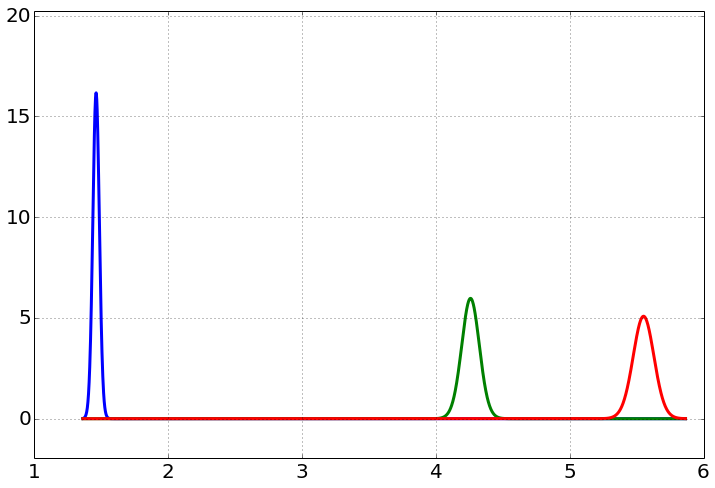
\includegraphics[width=4.5in]{Applications_of_Parameter_Estimation/Applications_of_Parameter_Estimation_fig0.png}\end{center}

\begin{lstlisting}
distplot(t_virginica)
\end{lstlisting}

\begin{center}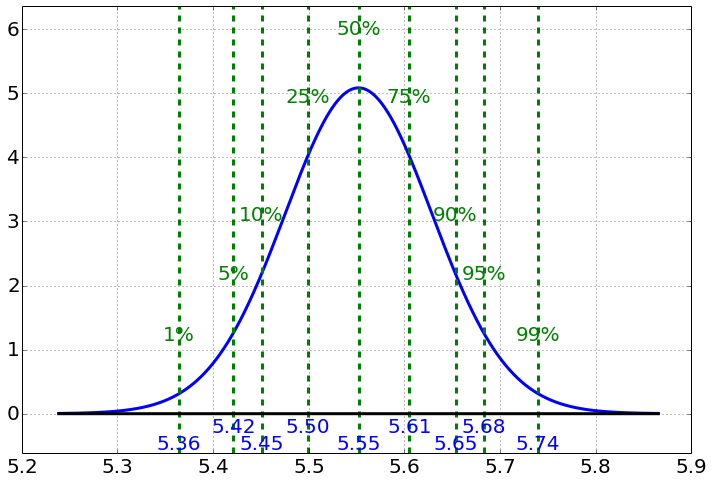
\includegraphics[width=4.5in]{Applications_of_Parameter_Estimation/Applications_of_Parameter_Estimation_fig1.png}\end{center}

\begin{lstlisting}
credible_interval(t_versicolor)
\end{lstlisting}

\begin{verbatim}
(4.1265203051077082, 4.2599999999999998, 4.3934796948922914)
\end{verbatim}

\begin{lstlisting}
credible_interval(t_virginica)
\end{lstlisting}

\begin{verbatim}
(5.3952325713636533, 5.5519999999999996, 5.7087674286363459)
\end{verbatim}

\subsection{Sunrise}


\begin{lstlisting}
dist=beta(h=365,N=365)
\end{lstlisting}

\begin{lstlisting}
distplot(dist)
\end{lstlisting}

\begin{center}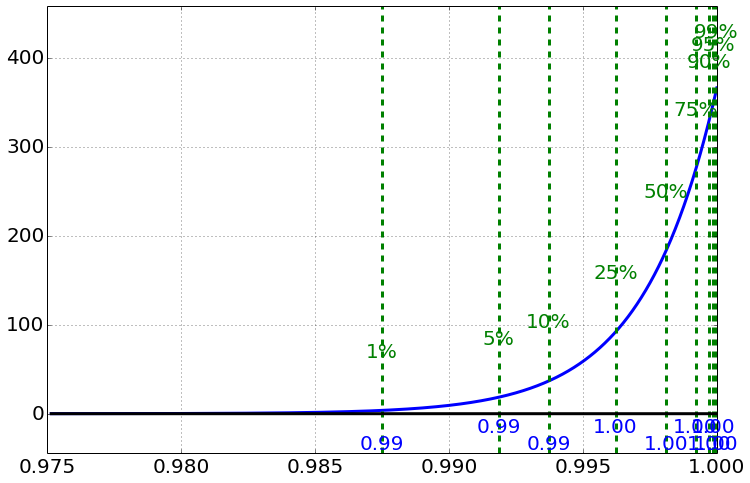
\includegraphics[width=4.5in]{Applications_of_Parameter_Estimation/Applications_of_Parameter_Estimation_fig2.png}\end{center}

\begin{lstlisting}
credible_interval(dist)
\end{lstlisting}

\begin{verbatim}
(0.98997171634278669, 0.99810794743679487, 0.99993082805373457)
\end{verbatim}

\subsection{Cancer Example}


\begin{lstlisting}
dist=beta(h=7,N=10)
\end{lstlisting}

\begin{lstlisting}
distplot(dist,figsize=(8,5))
\end{lstlisting}

\begin{center}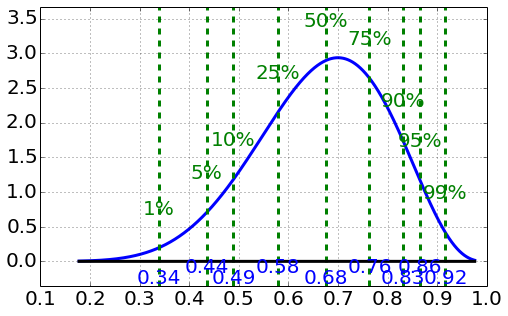
\includegraphics[width=4.5in]{Applications_of_Parameter_Estimation/Applications_of_Parameter_Estimation_fig3.png}\end{center}

\begin{lstlisting}
credible_interval(dist)
\end{lstlisting}

\begin{verbatim}
(0.39025744042757882, 0.67619553741481253, 0.89073655618090186)
\end{verbatim}

Essentially no evidence of any effect over 50 percent.

\subsection{Pennies}


\begin{lstlisting}
data1=load_data('data/pennies1.csv')
print data1
year,mass=data1['Year'],data1['Mass [g]']
\end{lstlisting}

\begin{verbatim}
    Year  Mass [g]
0   1960     3.133
1   1961     3.083
2   1962     3.175
3   1963     3.120
4   1964     3.100
5   1965     3.060
6   1966     3.100
7   1967     3.100
8   1968     3.073
9   1969     3.076
10  1970     3.100
11  1971     3.110
12  1972     3.080
13  1973     3.100
14  1974     3.093
\end{verbatim}

\begin{lstlisting}
plot(year,mass,'o')
xlabel('year')
ylabel('Mass per Penny [g]')
\end{lstlisting}

\begin{verbatim}
<matplotlib.text.Text at 0x1087c2d90>
\end{verbatim}

\begin{center}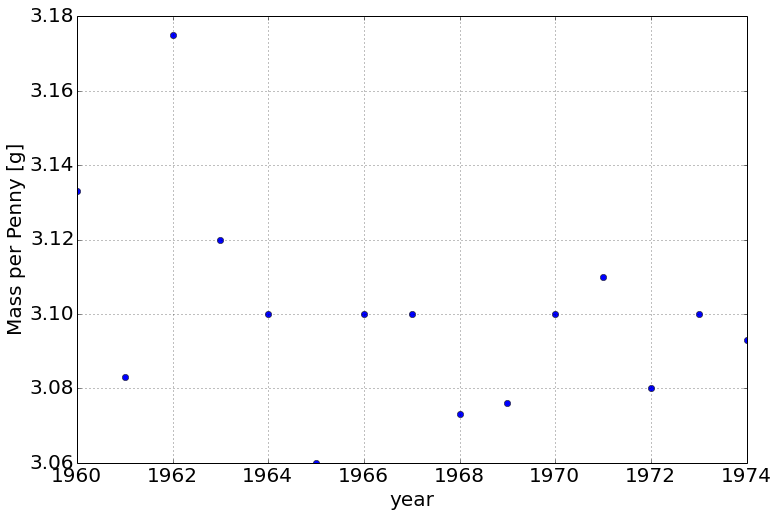
\includegraphics[width=4.5in]{Applications_of_Parameter_Estimation/Applications_of_Parameter_Estimation_fig4.png}\end{center}

\begin{lstlisting}
x=mass
mu=sample_mean(x)
N=len(x)
sigma=sample_deviation(x)/sqrt(N)
t_penny1=tdist(N,mu,sigma)

distplot(t_penny1,label='mass [g]')
\end{lstlisting}

\begin{center}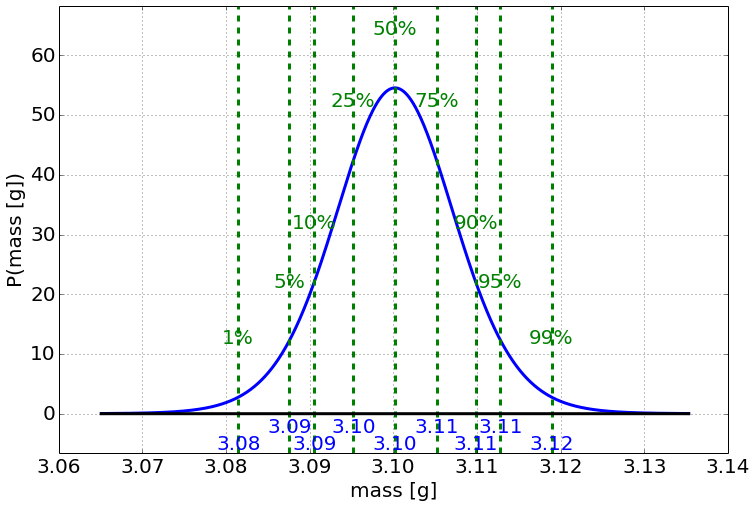
\includegraphics[width=4.5in]{Applications_of_Parameter_Estimation/Applications_of_Parameter_Estimation_fig5.png}\end{center}

\begin{lstlisting}
CI=credible_interval(t_penny1,percentage=99)
print CI
\end{lstlisting}

\begin{verbatim}
(3.0790129206702002, 3.1002000000000001, 3.1213870793298)
\end{verbatim}

\begin{lstlisting}
plot(year,mass,'o')
credible_interval_plot(t_penny1,percentage=99)
xlabel('year')
ylabel('Mass per Penny [g]')
\end{lstlisting}

\begin{verbatim}
<matplotlib.text.Text at 0x1087fcf10>
\end{verbatim}

\begin{center}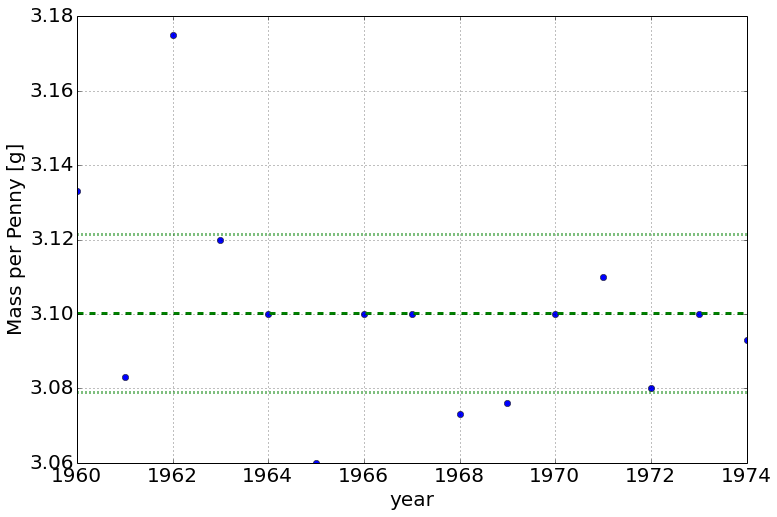
\includegraphics[width=4.5in]{Applications_of_Parameter_Estimation/Applications_of_Parameter_Estimation_fig6.png}\end{center}

\subsubsection{Do the 2 datasets}


\begin{lstlisting}
data2=load_data('data/pennies2.csv')
print data2
year1,mass1=year,mass
year2,mass2=data2['Year'],data2['Mass [g]']
\end{lstlisting}

\begin{verbatim}
    Year  Mass [g]
0   1989     2.516
1   1990     2.500
2   1991     2.500
3   1992     2.500
4   1993     2.503
5   1994     2.500
6   1995     2.497
7   1996     2.500
8   1997     2.494
9   1998     2.512
10  1999     2.521
11  2000     2.499
12  2001     2.523
13  2002     2.518
14  2003     2.520
\end{verbatim}

\begin{lstlisting}
x=mass1
mu=sample_mean(x)
N=len(x)
sigma=sample_deviation(x)/sqrt(N)
t_penny1=tdist(N,mu,sigma)

x=mass2
mu=sample_mean(x)
N=len(x)
sigma=sample_deviation(x)/sqrt(N)
t_penny2=tdist(N,mu,sigma)

distplot2([t_penny1,t_penny2],show_quartiles=False,label='mass [g]')
legend([r'$\mu_1$',r'$\mu_2$'])

\end{lstlisting}

\begin{verbatim}
<matplotlib.figure.Figure at 0x1087d3f10>\end{verbatim}

\begin{verbatim}
<matplotlib.legend.Legend at 0x1088198d0>
\end{verbatim}

\begin{center}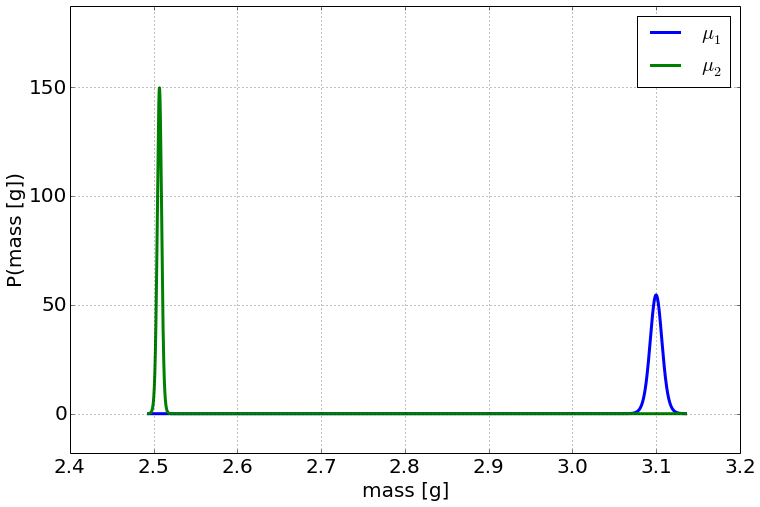
\includegraphics[width=4.5in]{Applications_of_Parameter_Estimation/Applications_of_Parameter_Estimation_fig7.png}\end{center}

\begin{lstlisting}
plot(year1,mass1,'o')
credible_interval_plot(t_penny1,percentage=99)
plot(year2,mass2,'ro')
credible_interval_plot(t_penny2,percentage=99,xlim=[1989,2005])
xlabel('year')
ylabel('Mass per Penny [g]')
\end{lstlisting}

\begin{verbatim}
<matplotlib.text.Text at 0x10907e310>
\end{verbatim}

\begin{center}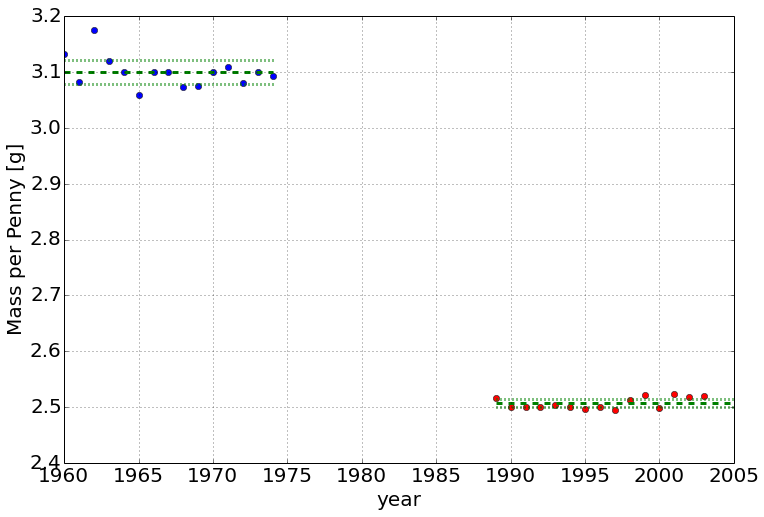
\includegraphics[width=4.5in]{Applications_of_Parameter_Estimation/Applications_of_Parameter_Estimation_fig8.png}\end{center}

\subsubsection{Distribution of the difference, normal approximation}


\begin{lstlisting}
N1=len(mass1)
N2=len(mass2)

mu1=sample_mean(mass1)
mu2=sample_mean(mass2)


sigma1=(1+20.0/N1**2)*sample_deviation(mass1)/sqrt(N1)
sigma2=(1+20.0/N2**2)*sample_deviation(mass2)/sqrt(N1)


delta_12=mu1-mu2
sigma_delta12=sqrt(sigma1**2+sigma2**2)

dist_delta=normal(delta_12,sigma_delta12)
distplot(dist_delta)
\end{lstlisting}

\begin{center}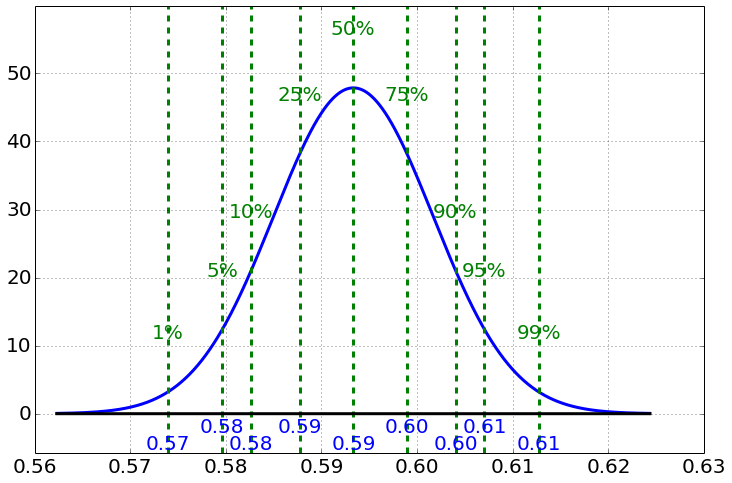
\includegraphics[width=4.5in]{Applications_of_Parameter_Estimation/Applications_of_Parameter_Estimation_fig9.png}\end{center}

clearly larger than zero at well over the 99% level.

\subsection{Ball Bearing Sizes}


\begin{lstlisting}
data1=[1.18,1.42,0.69,0.88,1.62,1.09,1.53,1.02,1.19,1.32]
data2=[1.72,1.62,1.69,0.79,1.79,0.77,1.44,1.29,1.96,0.99]
N1=len(data1)
N2=len(data2)
\end{lstlisting}

\begin{lstlisting}
mu1=sample_mean(data1)
mu2=sample_mean(data2)
print mu1,mu2
\end{lstlisting}

\begin{verbatim}
1.194 1.406
\end{verbatim}

\begin{lstlisting}
S1=sample_deviation(data1)
S2=sample_deviation(data2)
print S1,S2
\end{lstlisting}

\begin{verbatim}
0.289681817786 0.428309337849
\end{verbatim}

\begin{lstlisting}
sigma1=S1/sqrt(N1)
sigma2=S2/sqrt(N2)
print sigma1,sigma2
\end{lstlisting}

\begin{verbatim}
0.091605434094 0.135443305072
\end{verbatim}

\begin{lstlisting}
dist1=normal(mu1,sigma1)
dist2=normal(mu2,sigma2)
distplot2([dist1,dist2],show_quartiles=False,label='size [microns]')
legend([r'$\mu_1$',r'$\mu_2$'])
\end{lstlisting}

\begin{verbatim}
<matplotlib.figure.Figure at 0x105d61390>\end{verbatim}

\begin{verbatim}
<matplotlib.legend.Legend at 0x108ca1ad0>
\end{verbatim}

\begin{center}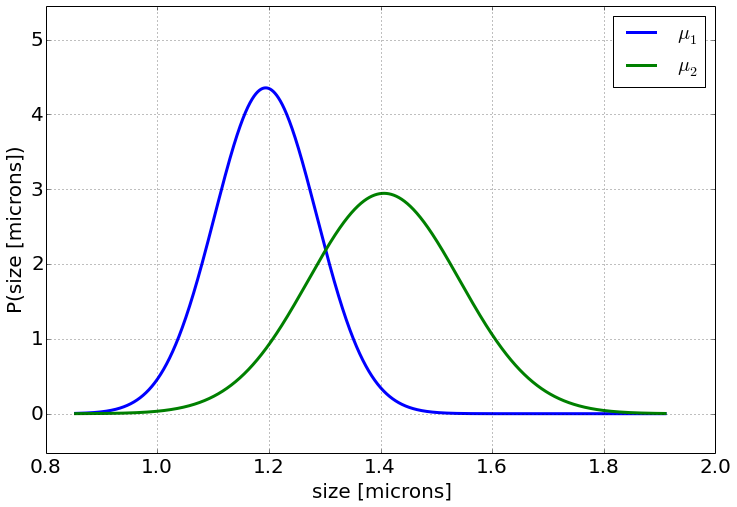
\includegraphics[width=4.5in]{Applications_of_Parameter_Estimation/Applications_of_Parameter_Estimation_fig10.png}\end{center}

\begin{lstlisting}

\end{lstlisting}


\end{fullwidth}
